%
\let\textcircled=\pgftextcircled
\chapter{Theory}
\label{chap:theory}

\section*{Contributions}\label{sec:theory_contributions}
This chapter represents a summary of existing work and contains no original contributions by the author of this thesis. 

\section{Introduction}
This chapter sets out the theory of Markov state models (MSMs) and hidden Markov models (HMMs) to describe the dynamics of biomolecular systems. Table \ref{tab:theory_symbols} summarises the  nomenclature used in this chapter. 

\begin{table}
    \centering
    \begin{tabularx}{0.9\textwidth}{ |l| >{\raggedright\arraybackslash}X | } 
        \hline
        \textbf{Symbol}  &  \textbf{Definition} \\
        \hline\hline
        $N_{\mathrm{A}}$ & Number of atoms. \\
        $N_{\mathrm{T}}$ & Number of trajectory frames. \\
        $N_{\mathrm{C}}$ & Number of important continuous features  \\
        $t$ & Time index or variable. \\
        $\mathbf{x}/\mathbf{y}(t)$ & Point in phase space as function of time. \\
        $\tau$ & Markov lag-time. \\
        $p(\mathbf{x}, \mathbf{y}; \tau)$ & Probability of observing $\mathbf{x}$ and then $\mathbf{y}$ a time $\tau$ later. \\
        $p(\mathbf{x}; t)$ & Probability distribution over phase space at time $t$. \\
        $\mu(\mathbf{x})$ & Stationary distribution of system in thermodynamic equilibrium.  \\ 
        $\mathcal{T}(\tau)$ & Transfer operator, equation \ref{eqn:transfer_operator}.  \\
        $q(\mathbf{x}; t)$ & Normalized descriptor of a thermodynamic ensemble. $q(\mathbf{x}) = \frac{p(\mathbf{x})}{\mu(\mathbf{x})}$. \\
        $(\psi_{i}(\mathbf{x}), \lambda_{i})$ & Eigenfunctions and eigenvalues of the transfer operator.  \\
        $r$ & The number of dominant eigenvalues: $\lambda_{2,\ldots, r}\simeq 1$ and $\frac{\lambda_{r}}{\lambda_{r+1}} \gg 1$. \\
        $n$ & Number of discrete states/microstates.\\
        $s^{i}\quad i = 1, \ldots, n$ & Indicator functions used to discretize phase space into $n$ states.  \\
        $\mathbf{s} = \{s_{1}, \ldots, s_{N_{T}}\} $ & Trajectory in the basis defined by $s^{i}$. \\
        $\mathbf{T}$ & Transition matrix. The discrete analogue of the transfer operator. \\
        $\bm{\pi}$ & Stationary distribution of the MSM. \\
        $\mathbf{p}(t)$ & State probability vector. Discrete analogue of $p(\mathbf{x}; t)$. \\
        $\mathbf{q}(t)$ & Normalized state vector. Discrete analogue of $q(\mathbf{x};t)$. \\
        $\mathbf{v}$ & Right eigenvectors of $\mathbf{T}$. Discrete analogue of $\psi_{i}(\mathbf{x})$. \\
        $\mathbf{u}$ & Left eigenvectors of $\mathbf{T}$. $\mathbf{u}$ and $\mathbf{v}$ are related by: $u_{i} = v_{i}\cdot\pi_{i}$ \\
        $\mathbf{X}$ & Data matrix.  Coordinates snapshots of trajectory: $\mathbf{X}\in \mathbb{R}^{N_{\mathrm{T}}\times N_{A}}$.\\
        $\bm{\chi}$ & Feature matrix. Transformation of $\mathbf{X}$ into important features of system. $\bm{\chi} \in \mathbb{R}^{N_{\mathrm{T}}\times N_{\mathrm{C}}}$. \\
        $\bm{\chi}^{\prime}$ & TICA transformed feature matrix. \\
        $\mathbf{C}$ & Time lagged correlation matrix between states. $C_{ij} = \mathrm{cor}(i, j; \tau)$  \\
        $\mathbf{c}$ & Count matrix for discrete states. $c_{ij} \propto C_{ij}$. \\
        $\mathbf{S}$ & Overlap matrix between  either continuous or discrete states. In the discrete basis, $\mathbf{S} = \diag{\{\bm{\pi}\}}$. \\
        $g$ & Number of hidden states of a HMM. \\
        $\mathbf{h} = \{h_t\}$ & Trajectory of hidden states. \\
        $\widetilde{\mathbf{T}}$ & Hidden state transition matrix of a HMM. \\
        $\widetilde{\bm{\pi}}$ & Hidden state stationary distribution of a HMM. \\
        $\mathbf{M}$ & Membership matrix of HMM. $M_{ji} = \mathbb{P}(h_t=i|s_t=j)$. \\
        $\mathbf{E}$ & Emission matrix of HMM. $E_{i, j}= \mathbb{P}(s_t=j|h_t=i)$. \\
     \hline
     \end{tabularx}
    \caption[Important symbols]{\textsc{Important symbols used throughout this chapter.}}

    \label{tab:theory_symbols}
\end{table}

\section{Markov processes}
Markov state models are now used routinely to quantitatively describe the conformational kinetics and thermodynamics of biomolecular systems using data collected from molecular dynamics simulations \cite{wangConstructingMarkovState2018c,noeMarkovModelsMolecular2019b}. A general, molecular system can be described by a vector of phase space coordinates  (momentum and position) as a function of time, $\mathbf{x}(t)$. A thermodynamic ensemble of such systems can be described by a probability density over $\mathbf{x}(t)$, $p(\mathbf{x}; t)$ \cite{prinzMarkovModelsMolecular2011}. Modelling a system in thermodynamic equilibrium as a Markov process imposes a number of assumptions on $p(\mathbf{x}; t)$ \cite{prinzMarkovModelsMolecular2011}:
\begin{enumerate}
    \item that there exists a period of time, $\tau$, over which the evolution of the system from a point $\mathbf{x}(t)$ to a new point $\mathbf{y}(t+\tau)$ is dependent only on $\mathbf{x}(t)$, i.e. the joint probability density $p(\mathbf{x}, \mathbf{y} ; \tau)$ is conditional \emph{only} on $\mathbf{x}$:
    \begin{equation}\label{eqn:markov_assumption}
    p(\mathbf{x}, \mathbf{y} ; \tau)=\mathbb{P}\left[\mathbf{x}(t+\tau) \in \mathbf{y}+d \mathbf{y} | \mathbf{x}(t)=\mathbf{x}\right].
    \end{equation}
    \item That there are no regions of phase space disconnected from one another, i.e. that the system is \emph{ergodic}. In this case there is a unique stationary distribution,  $\mu(\mathbf{x})$. At constant temperature $\mu(\mathbf{x})$ is the Boltzmann distribution. 
    \item The system is \emph{reversible} and so obeys detailed balance: 
    \begin{equation}\label{eqn:detailed_balance}
    \mu(\mathbf{x}) p(\mathbf{x}, \mathbf{y} ; \tau)=\mu(\mathbf{y}) p(\mathbf{y}, \mathbf{x} ; \tau), 
    \end{equation}
    in other words, the absolute probability of observing a transition from $\mathbf{x}$ to $\mathbf{y}$ (also known as the flux, $F(\mathbf{x}, \mathbf{y})$) is the same as that from $\mathbf{y}$ to $\mathbf{x}$. 
\end{enumerate}

The dynamics of a Markov process in continuous space is described by the \emph{transfer operator}, $\mathcal{T}(\tau)$, which propagates $q(\mathbf{x} ; t)$:
\begin{equation}\label{eqn:vector_norm}
    q(\mathbf{x} ; t) = \frac{p(\mathbf{x} ; t)}{\mu(\mathbf{x})},
\end{equation}
forward in time by \cite{prinzMarkovModelsMolecular2011}: 
\begin{equation}\label{eqn:transfer_operator}
\begin{split}
   q(\mathbf{y} ; t+\tau) &= \mathcal{T}(\tau) \cdot q(\mathbf{y} ; t) \\
   &=\frac{1}{\mu(\mathbf{y})} \int d \mathbf{x} p(\mathbf{x}, \mathbf{y} ; \tau) \mu(\mathbf{x}) q(\mathbf{x} ; t). 
\end{split}
\end{equation}

All the kinetic and thermodynamic information of the system is contained within $\mathcal{T}$, its eigenfunctions, $\psi_{i}(\mathbf{x})$, and eigenvalues $\lambda_{i}$, which, for reversible dynamics, all lie within the interval $-1 < \lambda_i \le 1$ \cite{schutteDirectApproachConformational1999}. The first eigenvector, with $\lambda_{1}=1$, is given by $\psi_{1}(\mathbf{x})=\mathbf{1}$ which corresponds to the stationary distribution $\mu(\mathbf{x})$ by virtue of the definition of $q(\mathbf{x})$, equation \ref{eqn:vector_norm} \cite{prinzMarkovModelsMolecular2011}. The remaining eigenvector/eigenvalue pairs shall be assumed to be ordered in decreasing value of $\lambda$.

The remaining eigenfunctions, $\psi_{2,3,4...}$, correspond to the relaxation processes which take the system from any initial distribution, $q(\mathbf{x} ; t=0)$ towards the stationary distribution on a timescale related to its corresponding eigenvalue \cite{prinzMarkovModelsMolecular2011}. This can be seen by writing the time evolution of $q(\mathbf{x};t)$ as:
\begin{equation}\label{eqn:eig_decomp}
q(\mathbf{x} ; t+k \tau)=\mathbf{1}+\sum_{i=2}^{\infty} e^{-k \tau / t_{i}}\left\langle q(\mathbf{x} ; t), \psi_{i}(\mathbf{x})\right\rangle_{\mu} \psi_{i}(\mathbf{x}),
\end{equation}
where $k=1,2,3 \ldots$ is a time index, and 
\begin{equation}
t_{i}=-\frac{\tau}{\ln{|\lambda_{i}|}}, 
\end{equation}
are the \emph{implied timescales} for the relaxation process described by $\psi_{i}(\mathbf{x})$ \cite{prinzMarkovModelsMolecular2011}. The bracketed quantity is the overlap between $q(\mathbf{x})$ and the eigenfunctions:
\begin{equation}
\left\langle q(\mathbf{x} ; t), \psi_{i}(\mathbf{x})\right\rangle_{\mu}=\int d \mathbf{x} \mu(\mathbf{x}) q(\mathbf{x} ; t) \psi_{i}(\mathbf{x}). 
\end{equation}

Each term in equation \ref{eqn:eig_decomp} will decay exponentially, and in the long time limit, as $k \rightarrow \infty$, leave just the first eigenvector, $\psi_{1}(\mathbf{x})=\mathbf{1}$, the stationary distribution. If the first $r$ eigenvalues are $\lessapprox 1$ and are separated from the remaining values by a gap such that $\lambda_{r} \gg \lambda_{r+1}$, then its possible to truncate equation \ref{eqn:eig_decomp}, without serious loss of accuracy, to:

\begin{equation}\label{eqn:eig_decomp_to_r}
q(\mathbf{x},  t+k \tau)  \simeq \mathbf{1}+\sum_{i=2}^{r} e^{-k \tau / t_{i}}\left\langle q(\mathbf{x} ; t), \psi_{i}(\mathbf{x})\right\rangle_{\mu} \psi_{i}(\mathbf{x}).
\end{equation}

These $r$ eigenfunctions are known as the \emph{dominant} eigenfunctions and they correspond to the slow relaxation processes of the system \cite{prinzMarkovModelsMolecular2011}. The truncation amounts to describing just the slow kinetic processes of the system while ignoring the fast processes. This separation of timescales implies the existence of regions of phase space, partitioned by the dominant eigenfunctions, known as \emph{metastable} states \cite{prinzMarkovModelsMolecular2011}.

\section{Markov state models}\label{sec:theory_msm}

Markov state models (MSMs) are discrete models of Markovian dynamics described in previous section \cite{prinzMarkovModelsMolecular2011}. The continuous quantities described above all have discrete analogues which will be described in detail in this section \cite{prinzMarkovModelsMolecular2011}:
\begin{itemize}
    \item The system is described by a set of $n$ discrete states denoted, $i=1, \ldots, n$. Instead of the continuous vector $\mathbf{x}(t)$, each trajectory is denoted by a vector of integers $\mathbf{s}$, where each component, $s_t$, is the state at time $t$. $t$ is now a discrete quantity, an integer multiple of the time-step, $\Delta t$, used to record the coordinates in an MD trajectory: $t=k\Delta t,\ k=1, 2, \ldots$. 
    \item The system can be described by a probability mass vector, $\mathbf{p}(t)$,  instead of a probability density function $p(\mathbf{x};t)$. The $i$th component of $\mathbf{p}(t)$ is the probability of the system being in  state $s^{i}$ at time $t$.
    \item The stationary distribution, $\bm{\pi}$, is defined by integrating the stationary distribution, $\mu(\mathbf{x})$, over the domain of each discrete state, $s^{i}$:
        \begin{equation*}
            \pi_{i}=\int_{\mathbf{x} \in s^{i}} \mathrm{d}\mathbf{x}\mu(\mathbf{x})
        \end{equation*}
    \item By analogy with equation \ref{eqn:vector_norm}, the system can also be described by $\mathbf{q}(t)$ where $q_{i} = p_{i}/\pi_{i}$.
    \item The time evolution of $\mathbf{q}(t)$ and $\mathbf{p}(t)$ is determined by the \emph{transition matrix}, $\mathbf{T}(\tau)$:
        \begin{align*}
            \mathbf{q}(t+\tau) &= \mathbf{T}(\tau) \cdot \mathbf{q}(t) \\
            \mathbf{p}^{\top}(t+\tau) & = \mathbf{p}^{\top}(t)\cdot \mathbf{T}(\tau)
        \end{align*}
    \item The eigenfunctions, $\psi(\mathbf{x})$, are now the right eigenvectors of $\mathbf{T}(\tau)$, $\mathbf{v}$, with the same interpretation. The left eigenvectors, $\mathbf{u}$, are related to the right eigenvectors by: $v_{i} = u_{i}/\pi_{i}$.  
 \end{itemize}

Creating an MSM starts with the collection of molecular dynamics (MD) data in the form of a set of short trajectories, with configurations saved every $\Delta t$ seconds. This thesis will consider only canonical ensemble simulations, using both over-damped Langevin dynamics \cite{ermakComputerSimulationCharged1974,ermakEquilibriumElectrostaticEffects1974} and velocity re-scaling \cite{bussiCanonicalSamplingVelocity2007} to maintain temperature. As a consequence, the momentum coordinates will be ignored as a feature for constructing MMs. 

If  each trajectory has $N_{\mathrm{T}}$ frames and $N_{\mathrm{A}}$ atoms then a trajectory can be represented by a data matrix, $\mathbf{X} \in \mathbb{R}^{N_{\mathrm{T}} \times 3N_{\mathrm{A}}}$. The trajectories  undergo a series of processing steps on the way to creating an MSM, these are \cite{noeMarkovModelsMolecular2019b, schererVariationalSelectionFeatures2019}: 
\begin{enumerate}
    \item \textbf{Create features:} A set of continuous features, the ``essential degrees of freedom'' \cite{schutteDirectApproachConformational1999}, $\chi_{i}, i \in \{1,\dots, N_{\mathrm{C}} \}$ are chosen to capture the slow dynamics of the system:
    \begin{equation*}
        \mathbf{X}  \rightarrow \bm{\chi},\quad \bm{\chi} \in \mathbb{R}^{N_{T} \times N_{C}}
    \end{equation*}
    Examples of continuous features include dihedral angles \cite{noeHierarchicalAnalysisConformational2007,choderaLongTimeProtein2006a,kubeCoarseGrainingMethod2007b,bucheteCoarseMasterEquations2008a}, residue contact distances \cite{stanleyKineticModulationDisordered2014,zhouDistributionReciprocalInteratomic2012,shuklaConformationalHeterogeneityCalmodulin2016}, root mean square deviation (RMSD) \cite{noe2009constructing,bowmanAtomisticFoldingSimulations2011a}, or secondary structure (SS) metrics \cite{muffKineticAnalysisMolecular2008}. Neither SS or RMSD are amenable to further dimensionality reduction (step \ref{step_dim_red}), but can be clustered (step \ref{step:cluster}) and so are included here. 
    \item \textbf{Dimensionality reduction:} The number of features is reduced still further by transforming $\bm{\chi}$ into a small number, $m$, of collective variables. 
    \begin{equation*}
        \bm{\chi}  \rightarrow \bm{\chi}^{\prime},\quad \bm{\chi}^{\prime} \in \mathbb{R}^{N_{\mathrm{T}} \times m}
    \end{equation*}
    This thesis will exclusively use time-lagged independent component analysis (TICA)  as a method of dimensionality reduction \cite{perez-hernandezIdentificationSlowMolecular2013a} \cite{schwantesImprovementsMarkovState2013}.\label{step_dim_red}
    \item \textbf{Discretization:} Each of the MD frames is assigned to one of $n$ different discrete states using a clustering algorithm such as k-means \cite{lloydLeastSquaresQuantization1982} clustering: 
    \begin{equation*}
        \bm{\chi}^{\prime} \rightarrow \mathbf{s},\quad \mathbf{s} \in \mathbb{Z}^{N_{\mathrm{T}}}
    \end{equation*}\label{step:cluster}
    \item \textbf{MSM estimation}: The transition matrix, $\mathbf{T}$, is estimated by counting transitions between discrete states separated by a time $\tau$. 
    \item \textbf{Coarse-graining:} The MSM is then coarse-grained by grouping the $n$ microstates into $g$ macrostates states. This thesis will exclusively consider hidden Markov models (HMMs) as a method for doing this. 
\end{enumerate}

\subsection{Create features}
The choice of continuous feature $\chi$ may be determined or at least strongly suggested by the question being asked and/or from prior knowledge of the system. However, since the introduction of variational scoring rules such as the GMRQ \cite{mcgibbonVariationalCrossvalidationSlow2015} and VAMP \cite{wuVariationalApproachLearning2020c}, they are typically chosen using cross-validation. This is discussed in depth in chapter \ref{chap:msm}. 

\subsection{Dimensionality reduction with TICA}\label{sec:theory_tica}

Dimensionality reduction using TICA was introduced as a preprocessing step for improving MSM construction \cite{perez-hernandezIdentificationSlowMolecular2013a, schwantesImprovementsMarkovState2013}. The result of a time-lagged independent component analysis is an estimate of the eigenvectors of the transfer operator. So if MD trajectories have been projected onto the contact distances of the protein, then the TICA eigenvectors are linear combinations of these distances such that the first component represents the equilibrium distribution, the second component represents the slowest relaxation process and so on. These are approximations to the true transfer operator eigenvectors because the true eigenvectors, in general, are non-linear in such features. If TICA is performed then the feature trajectories can be projected onto the first $m$ TICA components (where $m$ must be chosen), creating a new, smaller set of features. There are two advantages to this. First, the fact that the number of features has been reduced to $m$ dimensions, means that clustering will be more efficient. This is because the amount of computation required by k-means clustering, a popular approach to clustering,  scales with the number of dimension \cite{celebiComparativeStudyEfficient2013}, as was discussed in section \ref{sec:mm_applications} of the introduction to this thesis. The second, more important advantage, is that  if the TICA components are scaled by their eigenvalues (a process called kinetic mapping) then distances in the space of these components approximate \emph{kinetic distances} \cite{noeKineticDistanceKinetic2015}. The kinetic distance between two conformations correlates with how slowly they interconvert.  This means that geometric similarity now implies (at least approximately) kinetic similarity. Geometrically discretizing this space means that molecular dynamics frames which are all mapped to the same discrete state, will have similar rates of interconversion to other discrete states. This fulfills the main assumption behind approximating the dynamics of a system with a discrete master equation (see equation \ref{eqn:masterequation} of the introduction) \cite{zwanzigClassicalDynamicsContinuous1983a, noeTransitionNetworksModeling2008}.  


The TICA operator is a result of variationally optimising a set of continuous basis functions, $\chi_{i}$, to estimate the eigenfunctions, $\psi_{i}$, of the transfer operator. The method can be summarised as follows: a trial function, $f$, is expanded in the basis $\chi_{i}$: 
\begin{equation}\label{eqn:trial_func}
    f(\mathbf{x}) = \sum^{N_{\mathrm{C}}}_{i}a_{i}\chi_{i}(\mathbf{x})
\end{equation}
The variational principle for operators with bounded eigenvalues (such as the transfer operator) states that any approximate eigenfunction will have eigenvalues less than the true eigenvalues \cite{noeVariationalApproachModeling2013}. So choosing the coefficients $a_{i}$ to maximize the eigenvalues from using equation \ref{eqn:trial_func} will be the closest approximation to the true eigenfunctions that can be achieved with linear combinations of basis functions. Using the method of Lagrange multipliers to maximize the eigenvalues using $f(\mathbf{x})$ results in the following generalized eigenvalue equation \cite{nuskeVariationalApproachMolecular2014}: \begin{equation}\label{eqn:general_ev_equation}
    \mathbf{C}\mathbf{a} = \lambda \mathbf{S}\mathbf{a}
\end{equation}
Solving this equation requires estimating the matrix elements of $\mathbf{C}$ and $\mathbf{S}$. The elements of $\mathbf{C}$ are the time-lagged correlation functions ($\mathrm{cor}$) between $\chi_{i}$ and $\chi_{j}$ \cite{nuskeVariationalApproachMolecular2014}:
\begin{equation}
    \begin{split}
        C_{ij} =& \operatorname{cor}\left(\chi_{i}, \chi_{j}, \tau\right)\\
        =& \int \int \chi_{i}(\mathbf{z}) \mathbb{P}\left(\mathbf{x}(t+\tau)=\mathbf{z} \mid \mathbf{x}(t)=\mathbf{y}\right) \\
        & \times \chi_{j}(\mathbf{y}) \mathbb{P}\left(\mathbf{x}(t)=\mathbf{y}\right) \mathrm{d} \mathbf{y} \mathrm{d}\mathbf{z},        
    \end{split}
\end{equation}
which can be estimated from the MD trajectories. The matrix $\mathbf{S}$ is the overlap matrix whose elements are the scalar product between the basis functions, weighted by the stationary distribution \cite{nuskeVariationalApproachMolecular2014}:
\begin{align}
    S_{ij} &= \int \chi_{i}(\mathbf{x})\chi_{j}(\mathbf{x})\mu(\mathbf{x})^{-1} \mathrm{d}\mathbf{x}
\end{align}
Having solved for the TICA eigenvectors, keep the first $m$ columns of $\mathbf{a}$ and use this to transform feature matrix $\bm{\chi}$ \cite{perez-hernandezIdentificationSlowMolecular2013a,schwantesImprovementsMarkovState2013}:
\begin{equation}
    \bm{\chi}^{\prime} = \bm{\chi}\cdot[\mathbf{a}_{1}, \mathbf{a}_{2}, \cdots,  \mathbf{a}_{m}]
\end{equation}

\subsection{Discretization}
Discretization is performed on the $m$ dimensional feature matrix $\bm{\chi}^{\prime}$ using a clustering algorithm such as k-means or Ward clustering \cite{husicWardClusteringImproves2017a}. Each region of feature space, $S_{i}$, is assigned uniquely to the microstate $i$ through the associated indicator function, $s^{i}\left(\bm{\chi}^{\prime}\right)$ \cite{prinzMarkovModelsMolecular2011}:
\begin{equation}
s^{i}\left(\bm{\chi}^{\prime}\right)=\left\{\begin{array}{ll}
1, & \bm{\chi}^{\prime} \in S_{i} \\
0, & \bm{\chi}^{\prime} \notin S_{i}
\end{array}\right.
\end{equation}
To avoid introducing too many symbols, $s^{i}\left(\bm{\chi}^{\prime}\right)$ denotes the indicator functions, while $\mathbf{s}$ is the MD trajectory in the indicator function basis. The individual components of $\mathbf{s}$ will be denoted $s_{t}$ where $t$ is a time index. To highlight the time series nature of $\mathbf{s}$ it will sometimes denoted $\{s_{1}, s_{2}, \ldots \}$. 

\subsection{MSM estimation}
MSM estimation is analogous to TICA estimation but with  indicator basis functions $s^{i}$ replacing the continuous basis functions $\chi_{i}$ in equation \ref{eqn:trial_func} \cite{nuskeVariationalApproachMolecular2014}. The result of the optimisation of coefficients $a_{i}$ results in the same generalized eigenvalue expression, equation \ref{eqn:general_ev_equation}. Solving this equation is simplified by the fact that the indicator functions are orthogonal and so $S_{ij} = 0$ if $i \neq j$ and $S_{ii} = \pi_{i}$. Equation \ref{eqn:general_ev_equation} then becomes \cite{nuskeVariationalApproachMolecular2014,prinzMarkovModelsMolecular2011}:
\begin{align}\label{eqn:tran_def}
 \mathbf{C a}=\lambda \bm{\Pi} \mathbf{a} \\
\mathbf{T a}=\lambda \mathbf{a}   
\end{align}
where $\bm{\Pi} = \mathrm{diag}\{\pi_{1}, \ldots, \pi_{n}\}$ and $\mathbf{T} = \bm{\Pi}^{-1}\mathbf{C}$. In other words: 
\begin{equation}\label{eqn:tran_mat_def}
    T_{ij}(\tau) =\frac{\mathrm{cor}(s_{i}, s_{j}, \tau)}{\pi_{i}}
\end{equation}
For systems in thermodynamic equilibrium, the transition matrix elements must be estimated such that they respect the assumptions of i) reversibility and detailed balance, and ii) that the ergodicity i.e. that each state is connected to all other states \cite{nuskeVariationalApproachMolecular2014,prinzMarkovModelsMolecular2011}. Two methods exist for estimating $T_{ij}$: maximum likelihood estimation, MLE \cite{prinzMarkovModelsMolecular2011,bowmanProgressChallengesAutomated2009b}, and Bayesian estimation \cite{trendelkamp-schroerEstimationUncertaintyReversible2015b}. This work will make use of both: MLE will be used for model selection while Bayesian optimisation will be used when error estimates are required.  Detailed explanations of both  techniques can be in reference \cite{trendelkamp-schroerEstimationUncertaintyReversible2015b} but certain concepts need highlighting here: i) maximum likelihood estimation, ii) count matrices and ergodicity, iii) Bayesian estimation. 

\subsubsection{Maximum likelihood estimation}
Parameter estimation through maximum likelihood estimation proceeds by first modelling  the probability of observing the data $\{s_{1}, s_{2}, s_{3}, \ldots \}$ given \emph{fixed parameters}, $T_{ij}$ \cite{wasserman2013all}. For a MSM  with  $\tau=1$ this is \cite{trendelkamp-schroerEstimationUncertaintyReversible2015b}:
\begin{equation}\label{eqn:msm_traj_like}
    \mathbb{P}(\mathbf{s}|\mathbf{T}) \propto \prod_{t=1}^{N_{\mathrm{T}}} T_{s_{t}, s_{t+1}}
\end{equation}
The likelihood, $\mathcal{L}(\mathbf{T}|\mathbf{s})$, is equal $\mathbb{P}(\mathbf{s}|\mathbf{T})$ but treats the the \emph{data as fixed} and the \emph{parameters as varying}\footnote{The integral of the likelihood over the parameter space can be greater $1$ hence it is not a probability.} \cite{wasserman2013all}. Equation \ref{eqn:msm_traj_like} can be re-written in terms of the count matrix, $c_{ij}$, which counts all the observed transitions between states $i$ and $j$ \cite{trendelkamp-schroerEstimationUncertaintyReversible2015b}:
\begin{align}
    \mathcal{L}(\mathbf{T}|\mathbf{s}) & = \mathbb{P}(\mathbf{s}|\mathbf{T}) \\
    & \propto \prod_{t=1}^{n_{f}} T_{s_{t}, s_{t+1}} \\ 
    & \propto \prod_{i}\Pi_{j}T_{i, j}^{c_{ij}} \\
    & = \mathbb{P}(\mathbf{c}|\mathbf{T}) \label{eqn:msm_count_like}
\end{align}
So to calculate the maximum likelihood estimates (MLE) for $T_{ij}$, the count matrix $\mathbf{c}$ is estimated from the trajectories and then $T_{ij}$ are varied until a maximum value of $\mathcal{L}$ is found \cite{wasserman2013all}. For reversible MSMs an iterative scheme is used which ensures $\mathbf{T}$ satisfies detailed balance \cite{trendelkamp-schroerEstimationUncertaintyReversible2015b}. 


% As discussed in reference \cite{trendelkamp-schroerEstimationUncertaintyReversible2015b} the method for calculating the count matrix is important for estimating errors . In this case, correlation between frames means that pairs of states  This is typically the case in molecular dynamics simulations as molecular motions are correlated at short times and MD frames can be recorded with almost arbitrary temporal resolution .  


\subsubsection{Count matrix}\label{sec:theory_count_mat}
When the Markov lag-time is greater than the time-lag between frames, i.e., $\tau > 1\cdot \Delta t$, then there is ambiguity as to how the count matrix should be calculated. For accurate confidence intervals for the parameters $T_{ij}$ each pair of states, $(s_{t}, s_{t+\tau})$ should be independent \cite{trendelkamp-schroerEstimationUncertaintyReversible2015b}. The two extreme methods for counting are \emph{sliding window} and \emph{sample count} \cite{trendelkamp-schroerEstimationUncertaintyReversible2015b}. 

\emph{Sliding window} counts all pairs of frames separated by $\tau$: 
\begin{equation*}
    (s_0, s_{\tau}),\ (s_1, s_{1+\tau}),\ (s_2, s_{2+\tau})
\end{equation*}
For example, a trajectory with $N_{\mathrm{T}}=100$ frames, with $\tau=2$ has $\sum_{ij}c_{ij}=98$ observed transitions. If, as is usually the case with MD data, the observations are correlated at $t < \tau$, the confidence intervals generated will be too narrow, i.e., optimistic. 

The \emph{sample count} method uses the only the states separated by $\tau$:
\begin{equation*}
    (s_{0}, s_{\tau}),\ (s_{\tau}, s_{2\tau}),\ (s_{2\tau}, s_{3\tau})
\end{equation*}
Continuing the previous example, $\sum_{ij}c_{ij}=49$, a factor of $2$ different to the sliding window method. This leads to the confidence intervals being over-estimated. A third method, \emph{effective counting}, uses the sliding window method but scales count matrix elements by a factor, $I_{ij}$, to account for correlation between the observations \cite{noeStatisticalInefficiencyMarkov,trendelkamp-schroerEstimationUncertaintyReversible2015b}. Continuing the previous example, if the observations separated by $t<\tau$ are weakly correlated then the effective count matrix will be close to the sliding window estimate and $I_{ij} \lesssim 1$; if the observations are highly correlated the count matrix will be closer to the sample count method and $I_{ij}<1$. This method has been shown to give more accurate confidence intervals \cite{trendelkamp-schroerEstimationUncertaintyReversible2015b}. 

An MSM can only describe transitions between groups of microstates that are ergodic. For example, with \num{10} microstates, if no transitions are observed between a group consisting of microstates \num{1} and \num{2} and a group consisting of microstates \numrange[range-phrase=\text{--}]{3}{10} (but transitions are observed between all other pairs), then an MSM describes either the first group (a 2-state MSM results), or the second group (a 8-state MSM results).  However, the method of counting transitions between states, will determine whether or not those states are ergodic. There is a path between states $a$ and $z$ if there is a set of intermediate states, $b, c, \ldots, y$ such that $c_{a,b}>0,\ c_{b, c}>0,\ \ldots,\ c_{y, z}>0$. Two states are strongly or reversibly connected if there is a path from $a\rightarrow z$ and from $z\rightarrow a$. The full set of states are ergodic if each state pair of states is strongly connected \cite{wilson1996introduction}. The sliding window procedure utilises more transitions than the sample count method, and therefor will generally increase the size of the strongly connected set. In all estimation procedures used in this thesis, if the full set of state are not strongly connected, then a subset of states are used such that all states within the subset are strongly connected.

\subsubsection{Bayesian estimation}\label{sec:theory_bayes}
Bayesian estimation uses not just the likelihood, $\mathbb{P}(\mathbf{c}|\mathbf{T})$, but the prior probability of the parameters, $\mathbb{P}(\mathbf{T})$, to estimate the posterior probability of the parameters given the data, $\mathbb{P}(\mathbf{T}|\mathbf{c})$, using Bayes' rule \cite{gelmanBayesianDataAnalysis2014}: 
\begin{equation}
    \mathbb{P}(\mathbf{T}|\mathbf{c}) \propto \mathbb{P}(\mathbf{c}|\mathbf{T})\cdot\mathbb{P}(\mathbf{T})
\end{equation}
Rather than point estimates of the parameters, samples are drawn from the whole posterior distribution for each parameter, $T_{ij}$, using Markov chain Monte Carlo \cite{gelmanBayesianDataAnalysis2014}. These samples can then be used to estimate the distribution, and hence error, of any quantity determined by the transition matrix, e.g., eigenvalues or implied timescales \cite{gelmanBayesianDataAnalysis2014}. The details of the sampling procedures used for estimation of MSM in this work can be found in reference \cite{trendelkamp-schroerEstimationUncertaintyReversible2015b} and are implemented in the Python package PyEMMA (version 2.5) \cite{schererPyEMMASoftwarePackage2015a}, however two points should be highlighted here. First, the count matrices used are estimated using the effective count method. Second, the prior distribution for the transition matrix elements are defined over a reversible matrix $\mathbf{X}$, where $X_{ij}\propto T_{ij}\pi_{i}$, and is given by \cite{trendelkamp-schroerEstimationUncertaintyReversible2015b}: 
\begin{equation}\label{eqn:theory_rev_prior}
    \mathbb{P}(\mathbf{X}) \propto \Pi_{i \ge j}x_{ij}^{-1}. 
\end{equation}
This is to ensure the prior is consistent with detailed balance. As a result the posterior transition matrix elements have the same connectivity structure as the count matrix. i.e., if $c_{ij}=0$ then for any posterior sample $T_{ij}=0$ \cite{trendelkamp-schroerEstimationUncertaintyReversible2015b}. 

A method for testing the convergence of the MCMC sampling procedure is to calculate the rank-normalized $\hat{R}$ statistic using four independent sampling chains \cite{vehtariRanknormalizationFoldingLocalization2020}:
\begin{equation}
    \hat{R} = \frac{\hat{V}}{W}.
\end{equation}
Here $\hat{V}$ is the pooled variance of the four chains after rank normalization (i.e., sampled values are ranked and then the rank converted to a standard normal distributed variable) and $W$ is the within-chain variance. The recommended threshold value for convergence in reference \cite{vehtariRanknormalizationFoldingLocalization2020} is \num{1.01}, i.e if the sampling is converged then $\widehat{R} < 1.01$. The more stringent convergence tests in reference \cite{vehtariRanknormalizationFoldingLocalization2020} are not considered here due to the exploratory nature of this thesis.   

\subsection{Choice of Markov lag-time}
The lag time, $\tau$, is not a hyperparameter of the model but rather a part of the model specification; it defines the temporal resolution of the description of the dynamics. For large values of $\tau$ the truncation in equation \ref{eqn:eig_decomp_to_r} becomes more accurate, or, put another way, the Markov assumption becomes more plausible \cite{prinzMarkovModelsMolecular2011}. In addition, for small values of $\tau$ the correlation between the observations will mean that the transition matrix is non-Markovian, i.e., does not obey the Chapman-Kolmogorov equation \cite{wasserman2013all}:
\begin{equation}\label{eqn:ck_eqn}
[\mathbf{T}(\tau)]^{k} = \mathbf{T}(k \tau)
\end{equation}
However, if $\tau$ is too large then there may be processes of interest with timescales, $t_{i}<\tau$ which will not be captured \cite{prinzMarkovModelsMolecular2011}.

As a compromise, $\tau$ is chosen by inspection of the data through an \emph{implied timescale plot} \cite{prinzMarkovModelsMolecular2011,swopeDescribingProteinFolding2004a}. Starting from a given discrete trajectory, $\{s_{t}\}$ the implied timescales, $t_{i}$, are estimated for a range of different values of $\tau$. The lag time is chosen as the smallest $\tau$ such that $\frac{d t_{i}}{d \tau} \simeq 0$, where the range of $i$ is determined by the number of number slow relaxation processes. 

\subsection{Choice of hyperparameters}\label{sec:theory_choice_hyp}
The hyperparameters of the MSM are the modelling choices which transform the raw MD data into the $n$ discrete states, $s^{i}$, used in MSM estimation. This work will consider only the following hyperparameters: 
\begin{enumerate}
    \item $\chi$ the continuous feature,
    \item $\tau^{\prime}$ the TICA lag time ($\tau^{\prime}$ can be different from $\tau$), 
    \item $m$ the number of retained TICA components, 
    \item $n$ the number of cluster centers. 
\end{enumerate}
In principle, there are a large number of modelling choices which will have an effect on the final definition of the discrete states. These will described in the relevant sections later in this thesis. However, two important choices which will be kept fixed are: 
\begin{enumerate}
    \item the scaling of the TICA components. Each component will be scaled by their eigenvalues (the ``kinetic mapping'' option in PyEMMA \cite{schererPyEMMASoftwarePackage2015a});
    \item the k-means \cite{lloydLeastSquaresQuantization1982} algorithm will be used to cluster the TICA transformed trajectories into the discrete states. 
\end{enumerate}


Kinetic mapping is recommended for TICA dimensionality reduction \cite{noeKineticDistanceKinetic2015} because it maps geometric distances to kinetic distances (section \ref{sec:theory_tica}).  As already discussed in section \ref{sec:mm_applications} of the introduction to this thesis, a recent study looked at the quality of MSM models, created with different MSM hyperparameters \cite{husicOptimizedParameterSelection2016}, of twelve fast-folding proteins. The metric they used to judge model quality was the generalized matrix Rayleigh coefficient, which is discussed in full below, but essentially measures how accurately the  model describes the slow eigenvectors of the true transition matrix.  They found that on average using kinetic mapping with TICA increases the quality of the model compared to using TICA without kinetic mapping (which is in turn better than using PCA or no preprocessing). Kinetic mapping  mitigated the degradation in model quality introduced by including too many TICA components. However, this effect was smallest when using a small number of TICA components and for seven of the 12 optimum hyperparameters (the optimum for each protein) kinetic mapping was not used.  However, this may be due to the small number of scoring iterations used to estimate the model score: only five iterations were used, later studies on the same systems used \num{50} \cite{schererVariationalSelectionFeatures2019}. 

The choice of clustering algorithm has been investigated in reference \cite{husicWardClusteringImproves2017a} where the authors looked at the quality of MSMs, created using different clustering algorithms, of three of the twelve fast-folding proteins investigated in reference \cite{husicOptimizedParameterSelection2016}. They found that k-means and Ward clustering performed equivalently well when judged with the same model score used in reference \cite{husicOptimizedParameterSelection2016}.  K-means will be used in this work because of its good performance and the fact that it is implemented in the MSM package PyEMMA \cite{schererPyEMMASoftwarePackage2015a}. Fixing both the kinetic mapping and clustering algorithm reflects an arbitrary decision to keep the number of hyperparameters to a minimum.

The variational principle, used previously to optimize the coefficients in the basis function expansion, equation \ref{eqn:trial_func}, can also be used to optimize the basis functions themselves \cite{schererVariationalSelectionFeatures2019,husicOptimizedParameterSelection2016}. In order to do this objective functions known as the VAMP (variational approach to Markov processes) scores \cite{wuVariationalApproachLearning2020c} were derived which reach their upper limit when the resulting eigenfunctions become the exact eigenfunctions of the transfer operator. The VAMP scores generalize previous work on variationally optimising basis functions using the generalized matrix Rayleigh coefficient, GMRQ \cite{mcgibbonVariationalCrossvalidationSlow2015}. The VAMP scores are a family of scores, parameterized by an integer $w$ \cite{wuVariationalApproachLearning2020c}:
\begin{equation}\label{eqn:def_vampr}
\operatorname{VAMP}-w=\sum_{i=1}^{r}\left(\lambda_{i}\right)^{w}, 
\end{equation} 
where $r$ is the number of dominant eigenvalues of the transition matrix i.e. the $r$ in equation \ref{eqn:eig_decomp_to_r}. The GMRQ corresponds to $w=1$ and has been used to optimize parameters for MSMs of protein folding \cite{husicOptimizedParameterSelection2016}. This work will follow the suggestion in reference \cite{wuVariationalApproachLearning2020c} and a recent study which looked at selecting appropriate features for protein folding \cite{schererVariationalSelectionFeatures2019}. They used the VAMP score with $w=2$ (VAMP-2), which is equivalent to maximizing the kinetic variance \cite{wuVariationalApproachLearning2020c}. Maximizing the VAMP-2 score is then equivalent to choosing a basis set which most accurately describes the the slow dynamic processes of the system (see the earlier discussion of kinetic variance in section \ref{sec:theory_tica}). 

In order to use the VAMP-2 score the following steps can be used  \cite{schererVariationalSelectionFeatures2019}:
\begin{enumerate}
    \item select a set of hyperparameters to create a MSM basis, $s^{i}$, 
    \item estimate the MSM transition matrix, 
    \item calculate the VAMP-2 score, 
    \item repeat steps (1) - (3) a number of times until the VAMP-2 score converges.
\end{enumerate}
However, using equation \ref{eqn:def_vampr}, will tend to produce overly complex basis functions that fit to noisy fluctuations in the data, rather than the `true' relaxation processes \cite{mcgibbonVariationalCrossvalidationSlow2015,wuVariationalApproachLearning2020c,schererVariationalSelectionFeatures2019}, a process known as over-fitting \cite{friedman2001elements}.

Two popular techniques for mitigating over-fitting \cite{friedman2001elements} are the bootstrap \cite{efronIntroductionBootstrap1993} and cross-validation, CV \cite{arlotSurveyCrossvalidationProcedures2009}. The bootstrap consists of drawing samples (typically \num{100}s or \num{1000}s) from the data, with replacement, to form new data sets. Models are estimated and scored on these data. The distribution of model scores is used to calculate their mean and confidence intervals. Models can then be compared using these mean scores, which take into account an estimate of the sampling uncertainty. The idea of CV is to estimate the model parameters on a subset of the data, the training data $\mathcal{D}^{\mathrm{train}}$, and then evaluate the performance of the parameters on the remaining data $\mathcal{D}^{\mathrm{test}}$ \cite{friedman2001elements}. K-fold CV is popular for MSMs \cite{schererVariationalSelectionFeatures2019,mcgibbonVariationalCrossvalidationSlow2015}. In this method, the model is trained on $K-1$ disjoint `folds',  where a fold is \sfrac{1}{K} of the total data, e.g., if there are \num{100} MD trajectories, a fold will be \sfrac{100}{K} trajectories. The score is then evaluated on the single held out fold and the average score over the $K$ folds is used to evaluate the model. However, many different methods exist \cite{arlotSurveyCrossvalidationProcedures2009} and this work will use 50:50 shuffle split CV, which has been used previously for MSMs \cite{chenDynamicConformationalLandscape2019,husicOptimizedParameterSelection2016}. It is equivalent to repeated 2-Fold CV with a random permutation of the data in between each evaluation and is described in algorithm \ref{alg:shuffle_split}. 

\begin{algorithm}
\DontPrintSemicolon
\SetKwInput{Par}{Parameter}
\KwData{N independent trajectories: $\mathcal{D}=[\mathbf{s}_{1}, \mathbf{s}_{2}, \ldots, \mathbf{s}_{N}]$}

\KwIn{hyperparameter set: $\theta$}
\KwIn{estimator of model parameters: $P=P(\theta; \mathcal{D})$} 
\KwIn{scoring function: $CV(\theta) = CV(P;\mathcal{D})$}
\Par{number of iterations: $J$}
\BlankLine
\For{$i\leftarrow 1$ \KwTo $J$}{
    permute (``shuffle'') location  of trajectories  in $\mathcal{D}$: e.g., $\mathcal{D} \rightarrow [\mathbf{s}_{5}, \mathbf{s}_{17}, \ldots, \mathbf{s}_{2}]$\;
    split trajectories into two equal size, disjoint sets: $\mathcal{D} \rightarrow  \mathcal{D}^{\mathrm{train}},\quad \mathcal{D}^{\mathrm{test}}$\;
    estimate model parameters on training data: $P^{\mathrm{train}} = P(\theta,\mathcal{D}^{\mathrm{train}})$\;
    score model on test data: $CV^{\mathrm{test}}_{i} = CV_{i}(P^{\mathrm{train}}; \mathcal{D}^{\mathrm{test}})$\;
}
\KwResult{Cross-validated score: $\operatorname{MCV}(\theta)=\frac{1}{J}\sum_{i}CV^{\mathrm{test}}(\theta)$}
\caption{50:50 shuffle split cross-validation.\label{alg:shuffle_split}}
\end{algorithm}
It is important to note that for CV to judge the performance of all the hyperparameters, the `estimator of model parameters' must take as its input the \emph{raw} data \cite{friedman2001elements}. For the case of MSMs, the estimator takes the cartesian coordinates, applies TICA, clusters trajectories, and then estimates the transition matrix elements.  The scoring function, $CV$, for the VAMP-2 score is given by \cite{wuVariationalApproachLearning2020c}:
\begin{equation}
CV\left(\mathbf{C}, \mathbf{S}, \mathbf{v} \mid \mathcal{D}_{\text {test }}\right) 
=\left\|\left(\mathbf{v}^{\top} \mathbf{S}^{\text{test}} \mathbf{v}\right)^{-\frac{1}{2}}\left(\mathbf{v}^{\top} \mathbf{C}^{\text{test}} \mathbf{v}\right)\left(\mathbf{v}^{\top} \mathbf{S}^{\text{test}} \mathbf{v}\right)^{-\frac{1}{2}}\right\|_{2}^{2}
\end{equation}
where $\left\| \mathbf{A}\right\|_{2}^{2}$ is the square of the Frobenius norm of the matrix $\mathbf{A}$ \cite{wuVariationalApproachLearning2020c}. The matrices $\mathbf{S}^{\text{test}}$ and $\mathbf{C}^{\text{test}}$ are the overlap and time-lagged correlation matrices estimated on the test data, while $\mathbf{v}$ are the eigenvectors of the transition matrix estimated using the training data. 

\section{Coarse-graining with hidden Markov models}\label{sec:theory_hmm}
\subsection{HMM definition}
\begin{figure}
    \centering
    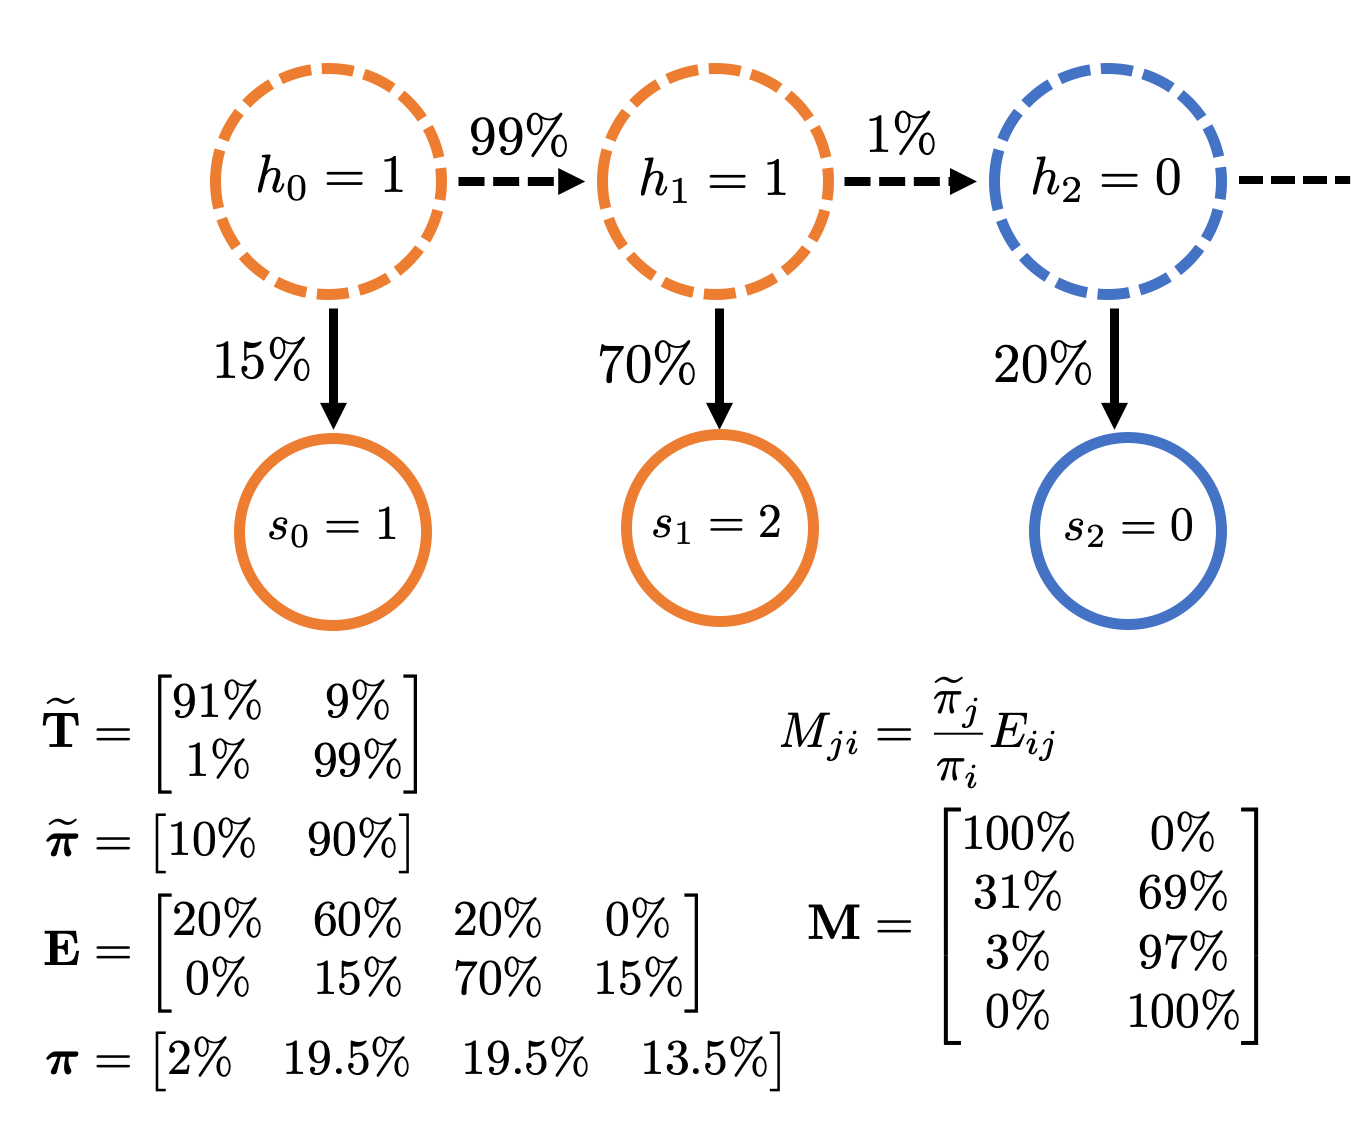
\includegraphics[width=0.8\textwidth]{chapters/theory/figures/hmm.png}
    \caption[Example hidden Markov model]{\textsc{Example hidden Markov model}. A schematic representation of a HMM with $g=2$ hidden states and $n=4$ observed states. The dashed circles represent the hidden states, the solid circles the observed states. Transition probabilities (from $\widetilde{\mathbf{T}}$) between hidden states label the dashed arrows; emission probabilities (from $\mathbf{E}$) label the solid arrows. }
    \label{fig:theory_hmm}
\end{figure}
Hidden Markov models (HMMs) are models of a dynamic process consisting of the following elements\footnote{This treatment focuses exclusively on discrete hidden Markov processes.} \cite{rabinerTutorialHiddenMarkov1989}:
\begin{enumerate}
    \item A number of hidden states, $g$. These are not observed in the data used to train the model.  
    \item Hidden-state to hidden-state transition probabilities, $\mathbb{P}(h_{t+1}|h_{t})$, where $h_{t}$ is the hidden state at time $t$. These are encoded in the hidden state transition matrix, $\widetilde{\mathbf{T}}\in \mathbb{R}^{g \times g}$. This has the same interpretation as the MSM transition matrix, $\mathbf{T}$. In keeping with the notation of reference \cite{noeProjectedHiddenMarkov2013a}, the $\ \widetilde{}\ $ pertains hidden quantities. 
    \item A number of observed states, $n$. These are the observations used to train the model. 
    \item Probabilities of seeing the observed states, given a hidden state. These encoded in the `emission matrix', $\mathbf{E}$, where  $E_{ij} = \mathbb{P}(s=j|h=i)$.  
    \item An initial distribution of hidden states, $\widetilde{\bm{\pi}}^{\prime}$.
\end{enumerate}

An example HMM is shown in figure \ref{fig:theory_hmm}. The hidden states are shown in dashed circles and the hidden-state to hidden-state transition probability label the dashed arrows. These are taken from the transition matrix $\widetilde{\mathbf{T}}$ shown. The stationary distribution, $\widetilde{\bm{\pi}}$, ensures detailed balance:
\begin{align*}
    \widetilde{T}_{1,2}\times \widetilde{\pi}_{1} & = \widetilde{T}_{2,1}\times \widetilde{\pi}_{2}\\
    0.09\times 0.1 & = 0.9 \times 0.01
\end{align*}
While in each hidden state the system emits to a observed state shown as solid circles and the emission probabilities label the solid arrows. These are taken from the  emission matrix $\mathbf{E}$ shown. Other quantities of interest are the observed state distribution $\bm{\pi}$ which is related to the emission and  stationary distribution by $\pi_{j} = \sum_{i}E_{ij}\widetilde{\pi}_{i}$;  and the membership matrix, $\mathbf{M}$. The membership matrix encodes the probability of the system being in an hidden state given the observed state \cite{noeProjectedHiddenMarkov2013a}, i.e., $M_{ji}=\mathbb{P}(h=i|s=j)$. This can determined from the stationary distributions of the hidden states and observed states, the emission matrix and the laws of probability:
\begin{align}
    \mathbb{P}(h=i|s=j) &= \frac{\mathbb{P}(h=i)}{\mathbb{P}(s=j)}\mathbb{P}(s=j|h=i) \\
    M_{ji} &= \frac{\widetilde{\pi}_j}{\pi_i}E_{ij}
\end{align}
The eigenvalues and eigenvectors of the hidden transition matrix have a similar interpretation as the eigenvectors and eigenvalues of an MSM, i.e., they are the relaxation processes and associated timescales, respectively, of the hidden states. 

\subsection{Coarse-graining procedure}\label{sec:theory_coarse_grain}
HMMs have been proposed as a method for modelling biomolecular dynamics by coarse-graining a MSM \cite{noeProjectedHiddenMarkov2013a}. This coarse-graining is accurate under the following assumptions \cite{noeProjectedHiddenMarkov2013a}:
\begin{enumerate}
    \item The underlying dynamics of the system are Markovian, i.e. they can be modelled by a transfer operator, $\mathcal{T}(\tau)$ (equation \ref{eqn:transfer_operator}). 
    \item There is a gap between the $r$'th and $r+1$'th  eigenvalues of $\mathcal{T}(\tau)$ i.e. $\frac{\lambda_{r}}{\lambda_{r+1}} \gg 1$.\label{assump_two}
    \item The $r$ dominant eigenfunctions partition the stationary distribution into $r$ metastable states. The probability of the system being in the boundary between these sets is negligible. \label{assump_three}
\end{enumerate}

The process for coarse-graining an MSM is as follows (adapted from algorithm 1 in \cite{noeProjectedHiddenMarkov2013a}): 
\begin{enumerate}
    \item \textbf{Estimate an MSM}. Using the process described in section \ref{sec:theory_msm}, transform the raw MD trajectories, $\{\mathbf{X}_{1}, \mathbf{X}_{2}, \ldots\}$, into trajectories of discrete states, $\{\mathbf{s}_{1},\mathbf{s}_{2}, \ldots\}$. Using these discrete trajectories estimate the MSM transition matrix, $\mathbf{T}$ at a lag-time $\tau$. 
    \item \textbf{Determine number of metastable states}. The number of metastable states, $r$, is determined by looking for a gap in the eigenvalues of $\mathbf{T}$, such that  $\frac{\lambda_{r}}{\lambda_{r+1}} \gg 1$. \emph{The number of hidden states of the HMM, $g$, is equal to the number of metastable states, $r$}.\label{item:theory_nmetastable}
    \item \textbf{Coarse-grain the transition matrix}. Estimate initial HMM parameters, $\widetilde{\mathbf{T}}_{0}$,  $\mathbf{E}_{0}$ and $\widetilde{\bm{\pi}}^{\prime}_{0}$, using robust PCCA \cite{deuflhardRobustPerronCluster2005b}. 
    \item \textbf{Estimate the HMM}. Optimise the HMM parameters (maximize the likelihood) using the Baum-Welch algorithm \cite{baumMaximizationTechniqueOccurring1970,welch2003hidden}, which is described in the next section. 
\end{enumerate}

Robust PCCA (or PCCA+) effectively utilises the sign structure of the dominant eigenvectors of the MSM in the microstate basis to assign microstates to metastable states. For example, if there are $r=3$ dominant eigenvalues (including the $\lambda = 1$ eigenvalue corresponding to the stationary distribution) identified in step \ref{item:theory_nmetastable}, then PCCA+ will partition the microstates into three metastable states. The method for assigning microstates to metastable states is as follows (this follows the description given in reference \cite{bowmanQuantitativeComparisonAlternative2013} assuming grouping into three metastable states): for each microstate $i$, create a vector $\mathbf{v}^{i}=(q^{i}_{1}, q^{i}_{2}, q^{i}_{3})$ where $q_{k}$ are the values of the $k$th eigenvector for that microstate. From among all the $\mathbf{v}^{i}$ choose three that are the most distinct from one another (using the Gram-Schmidt orthonormalisation algorithm). These three states are assigned to the three metastable states.  Assign the remaining microstates to either of these three metastable states based on their similarity to the three representative vectors $\mathbf{v}^{i}$. 

The $g$ eigenvalues and $g-1$ relaxation processes of the HMM will be the coarse-grained equivalent of the  eigenvalues and eigenvectors measured in the MSM basis \cite{noeProjectedHiddenMarkov2013a}. 

\subsection{HMM estimation}

\begin{algorithm}
\DontPrintSemicolon
\SetKwInput{Par}{Parameter}
\KwData{Initial HMM parameters: $\theta_{0} = (\widetilde{\mathbf{T}}_{0}$,  $\mathbf{E}_{0}$, $\widetilde{\bm{\pi}}^{\prime}_{0})$}
\KwData{observed state trajectory: $\{s_t\}$, $t = 1, \ldots, N_{\mathrm{T}}$}
\Par{likelihood tolerance: $\epsilon$}
\BlankLine
\Begin{
$\mathrm{ll_{0}},\ \theta,\ \mathrm{continue}   \longleftarrow 0,\ \theta_{0},\ \mathtt{True} $\;
\While{$\mathrm{continue}$}{
    \textbf{Forward procedure}\;
    Calculate the probability of being in hidden state $i$ at time $t$ and seeing the partial trajectory $s_1, \ldots, s_{t^{\prime}}$, given the model parameters:\;
    \begin{equation*}
      \alpha_i(t) = \mathbb{P}(\{s_{1}, \ldots, s_{t}\}| h_t=i, \theta)  
    \end{equation*}
    \textbf{Backward procedure}\;
    Calculate the probability of seeing the partial trajectory $s_{t+1}, \ldots, s_{N_{\mathrm{T}}}$, given being in hidden state $i$ and the model parameters, $\theta$:\;
    \begin{equation*}
     \beta_i(t) = \mathbb{P}(\{s_{t+1}, \ldots, s_{N_{\mathrm{T}}}\}|h_{t}=i, \theta)   
    \end{equation*}
    
    \textbf{Update model parameters}\;
    Calculate probability of being in hidden state $i$ at time $t$ given the entire trajectory $\{s_{t}\}$ and  $\theta$:\;
    \begin{equation*}
    \gamma_{i}(t) = \mathbb{P}(h_t=i|\{s_t\}, \theta) = \frac{\alpha_{i}(t) \beta_{i}(t)}{\sum_{j=1}^{g} \alpha_{j}(t) \beta_{j}(t)}
    \end{equation*}
    Calculate probability of begin in hidden state $i$ and time $t$ and transitioning to state $j$ at time $t+1$ given the entire trajectory $\{s_{t}\}$ and  $\theta$:\;
    \begin{equation*}
        \xi_{ij}(t) = \mathbb{P}(h_t=i, h_{t+1} = j|\{s_t\}, \theta) = \frac{\alpha_{i}(t)T_{ij}\beta_{j}(t+1)E_{j, s_{t+1}}}{\sum_{k, l}^{g}\alpha_{k}(t)T_{kl}\beta_{l}(t+1)E_{l, s_{t+1}}}
    \end{equation*}
    Update parameters using:
    \begin{align*}
        \widetilde{\pi}_{i}^{\prime}  &\longleftarrow \gamma_{i}(t=1) \\
        \widetilde{T}_{ij} & \longleftarrow \frac{\sum_{t=1}^{N_{T}-1} \xi_{i j}(t)}{\sum_{t=1}^{N_{T}-1} \gamma_{i}(t)} \\
        E_{ij} & \longleftarrow \frac{\sum_{t=1}^{N_{T}} 1_{s_{t}=j} \gamma_{i}(t)}{\sum_{t=1}^{T} \gamma_{i}(t)} \\
        \theta & \longleftarrow (\widetilde{\bm{\pi}}^{\prime}, \widetilde{\mathbf{T}}, \mathbf{E})
    \end{align*}
    \textbf{Calculate log-likelihood}\;
    $\mathrm{ll}^{\prime} = \log{\left(\sum_{i}^{g}\alpha_{i}(N_{T})\right)}$\;
    \If{$\mathrm{ll}^{\prime}-\mathrm{ll} < \epsilon$}{
        $\mathrm{continue} \longleftarrow \mathtt{False}$}
    $\mathrm{ll} \longleftarrow \mathrm{ll}^{\prime}$\;
}
}
\caption{The Baum-Welch algorithm.}\label{alg:baum_welch}
\end{algorithm}

The Baum-Welch algorithm as used for coarse-graining reversible MSMs is given in detail in reference \cite{noeProjectedHiddenMarkov2013a}. The algorithm is sketched in algorithm \ref{alg:baum_welch} to introduce some of the important quantities used later in this thesis. In particular, the `forward' part of the algorithm calculates the $\alpha_{i}(t)$ variable which is the probability of arriving at hidden state $i$ at time $t$ \emph{and} seeing the actual observed trajectory up to that point \cite{rabinerTutorialHiddenMarkov1989}. Summing this value for $t=N_{\mathrm{T}}$ over the hidden states gives the probability of the observed trajectory given the model parameters \cite{rabinerTutorialHiddenMarkov1989}. This is equal to the likelihood of the parameters given the observed trajectory, $\mathbb{P}(\{s_{t}\}|\theta)=\mathcal{L}(\theta|\{s_{t}\})$ \cite{rabinerTutorialHiddenMarkov1989}. 

In addition to the maximum likelihood estimation of the parameters, Bayesian estimation can be used. The details of the implementation used in PyEMMA (version 2.5) \cite{schererPyEMMASoftwarePackage2015a} can be found in reference \cite{choderaBayesianHiddenMarkov2011a} and the references therein, but the broad outline for estimating a Bayesian HMM with $g$ hidden states is as follows:
First, an MSM is estimated and the implied timescales, $t_{2},t_{3}, \ldots$, saved. Second, the trajectories are sub-sampled, or strided, to account for the correlation between observed states. The striding is by a factor $\Delta t$ given by \cite{schererPyEMMASoftwarePackage2015a}:
\begin{equation}\label{eqn:hmm_striding}
    \Delta t = \min{\left(\tau, 2\cdot t_{g+1}\right)}. 
\end{equation}
i.e., if $g=5$ the HMM will  capture the first five timescales in the full MSM basis. The $6$th implied timescale measured in the MSM basis will the slowest relaxation timescale but which is nevertheless considered too fast to be included in the HMM. This is analogous to the expression given in reference \cite{noeStatisticalInefficiencyMarkov}.  This means only the following transition are counted: 
\begin{equation}
    \left\{(s_{0}, s_{\tau}),\ (s_{\Delta t}, s_{\Delta t + \tau})\ \ldots \right \}.
\end{equation}

Third, a maximum likelihood HMM is estimated and is used to i) determine the largest strongly connected set of hidden states and ii) define the prior distribution of  $\widetilde{\bm{\pi}}^{\prime}$. The count matrix of the maximum likelihood model is determined by $\xi_{ij}$ from the Baum-Welch algorithm. The largest connected set is defined the same way as for the MSM case. 

Fourth, the parameters are sampled using MCMC. The prior function for $\widetilde{\mathbf{T}}$ is given by equation \ref{eqn:theory_rev_prior} and for $\widetilde{\bm{\pi}}^{\prime}$ is given by: 
\begin{equation}
    \widetilde{\bm{\pi}}^{\prime} \sim \prod_{i} \widetilde{\pi}_{0, i}^{a_{i}+n_{i}-1},
\end{equation}
where $a_{i}$ are the initial distribution from the maximum likelihood model and $n_{i}$ is the population of each hidden state at each sampling step in the MCMC algorithm. No priors for the emission distributions are used, instead the values of are determined from the other sampled quantities. Convergence of the parameters is performed in the same manner as for the MSM, i.e., through sampling independent chains and calculating the $\hat{R}$ statistic. 

\section{Markov model validation}\label{sec:model_validation}
Markov model validation for both MSMs and HMM is performed by checking to see if the Chapman-Kolmogorov equation,
\begin{equation}
[\mathbf{T}(\tau)]^{k} \approx \mathbf{T}(k \tau),
\end{equation}
holds to within sampling error for a range of $k$. This check is called the \emph{Chapman-Kolmogorov test} (CK test) \cite{prinzMarkovModelsMolecular2011}.  The left-hand side is a transition matrix \emph{predicted at time $k\tau$} from the matrix estimated at time $\tau$. The right hand-side is the transition matrix \emph{estimated at time $k\tau$}. This equality will hold exactly for a discrete Markov process (i.e., one for which there was no error in creating the discretized states, $s^i$ \cite{prinzMarkovModelsMolecular2011}). For an MSM, testing equality of two $n \times n$ transition matrices requires $n^{2}$ comparisons which is both computationally intractable and would result in large uncertainties \cite{prinzMarkovModelsMolecular2011}. Instead, the MSM is coarse-grained as a HMM and the CK test adapted as follows \cite{prinzMarkovModelsMolecular2011}:
\begin{enumerate}
    \item For each value of $k = 1, 2, 3, \ldots$ calculate $\widetilde{\mathbf{T}}(
    k\tau)$
    \item Using an initial state vector $\mathbf{p}(0)$ and $\widetilde{\mathbf{T}}(\tau)$ predict the values of $\mathbf{p}(k\tau)$ using: 
    \begin{equation*}
        \mathbf{p}^{\top}(k\tau)_{\mathrm{HMM}} = \mathbf{p}(0)^{\top}[\widetilde{\mathbf{T}}(\tau)]^{k}
    \end{equation*}
    \item Now predict $\mathbf{p}(k\tau)$ from the same initial state using the  $\widetilde{\mathbf{T}}(k\tau)$ matrices: 
    \begin{equation*}
        \mathbf{p}^{\top}(k\tau)_{\mathrm{Trajectory}} = \mathbf{p}(0)^{\top}\widetilde{\mathbf{T}}(k\tau)
    \end{equation*}
    \item Compare the $\mathbf{p}(k\tau)_{\mathrm{HMM}}$ and $\mathbf{p}(k\tau)_{\mathrm{Trajectory}}$ for a range of values of $k$ and for different initial state vectors, $\mathbf{p}(0)$. In PyEMMA (version 2.5) \cite{schererPyEMMASoftwarePackage2015a} $\mathbf{p}(0)$ are the HMM basis vectors, i.e. $\mathbf{p} = (1, 0, 0, \ldots),\ (0, 1, 0, \ldots)$. 
\end{enumerate}


\section{Summary}
This chapter has described the theory underlying constructing Markov state models in a fine grained microstate basis and then coarse-graining this model using hidden Markov models. To summarise the methods detailed here, starting from a set of molecular dynamics trajectories.  \emph{Step 1}: choose a feature, $\chi$, related to the slow dynamic processes being studied and project the atomic coordinates of the trajectories onto this feature. \emph{Step 2}: perform a time-lagged independent component analysis (TICA) parameterized with a lag time of $\tau^{\prime}$, and project the feature trajectories onto the first $m$ TICA components. This step is optional and is not used in the work of chapter \ref{chap:water} which estimates Markov models of water dynamics in aerosol particles. \emph{Step 3}: cluster the reduced dimension trajectories into $n$ microstates used k-means clustering. \emph{Step 4}: determine an appropriate Markov lag time by estimating Markov state models at different lag times and looking for the smallest lag such that the slow implied timescales remain constant. \emph{Step 5}: estimate a Markov state model at this lag time, $\tau$, and determine the number of dominant processes, $r$, by looking for gaps in eigenvalue spectrum of $\mathbf{T}(\tau)$. This model is then specified by the hyperparameters $(\chi,\tau^{\prime}, m, n)$.  \emph{Step 6}: Score this model by calculating the cross-validated VAMP-2 score using the $r$ dominant eigenvectors.  \emph{Step 7}: repeat steps $1-3$ varying the values of the hyperparameters and re-scoring the resulting models, while keeping the number of dominant eigenvectors, $r$,  and the Markov lag time, $\tau$, fixed. Then choose the set of hyperparameters which maximize the VAMP-2 score.  A more efficient method for performing these steps, utilising ideas from the machine learning community, is investigated in chapter \ref{chap:msm} using the benchmark system of alanine dipeptide. \emph{Step 8}: coarse-grain the optimum MSM using a hidden Markov model with $r$ hidden states representing the $r$ metastable states, as determined in step 5.  In chapter \ref{chap:hmm} a different method for determining the number of metastable states is investigated. This method uses more abstract classification techniques taken from the statistics community and tests them on a model four-well system.  Chapter \ref{chap:aadh} incorporates the work of chapters \ref{chap:msm} and \ref{chap:hmm} into this general method in order to develop a Markov model description of the conformational dynamics of the enzyme aromatic amine dehydrogenase. 

% To ensure the  measured response was generalisable \cite{friedman2001elements}, $20$ iterations of 50:50 shuffle split cross validation were used \cite{husicOptimizedParameterSelection2016}. For each trial this entailed fitting a model using \SI{50}{\percent} of the available data (the training data) with the following pipeline:

% \begin{enumerate}
%     \item \label{lst:modfititem1} The Cartesian coordinates were projected onto the required feature, $\chi$. 
%     \item \label{lst:modfititem2} For features (1) - (4) in AADH, TICA was applied with a lag time $\tau$ and the first $m$ independent  components were retained. 
%     \item \label{lst:modfititem3} k-means clustering \cite{friedman2001elements} was used to cluster the the frames in the TICA space into $n$ microstates.
%     \item \label{lst:modfititem4} A reversible, maximum likelihood Markov state model was estimated using these discrete trajectories. 
% \end{enumerate}

% The model was then scored on the remaining \SI{50}{\percent} (the test data) using the same pipeline without re-estimating the various model parameters (the expression for calculating the cross validated $\operatorname{VAMP}$ scores is described in \cite{mcgibbonVariationalCrossvalidationSlow2015} and \cite{wuVariationalApproachLearning2019}). This was repeated $20$ times, shuffling the trajectories in between each iteration [TM: Explain this].  The final trial response was calculated as the mean of the scores on the test data. All MSM fitting and MD trajectory analysis was performed in Python 3.7 using the packages PyEMMA \cite{schererPyEMMASoftwarePackage2015a}, MDTraj \cite{mcgibbonMDTrajModernOpen2015}, NumPy \cite{waltNumPyArrayStructure2011}, Pandas \cite{mckinneyPandasFoundationalPython2011}, Matplotlib \cite{hunterMatplotlib2DGraphics2007},  Seaborn \cite{michaelwaskomMwaskomSeabornV02020} and the Jupyter Project \cite{kluyverJupyterNotebooksPublishing2016} [TM: add version numbers].

% \subsubsection{Choice of $m$}
% With optimal choices of the hyperparameters and lag time the transition matrix represents a complete description of the dynamics of the system. In order to extract chemical significance from the transition matrix we must cluster the microstates into the metastable states of the system. This means:
% 1. choosing the number of metastable states deciding how many metastable states there are (the value of $m$ ) and;
% 2. assigning a probability for being in metastable state $i$ given we observe the system in state $s_{i}$, summarized in a membership matrix (equation 4-6).
% As with the choice of $s,$ pre-existing knowledge may constrain that choice but a simple data driven way of determining $m$ is to look at the ratio of successive eigenvalues ( $\lambda_{i} / \lambda_{i+1}$ ) or implied timescales $\left(t_{i} / t_{i+1}\right)$ and choose $m$ such that:
% \begin{equation}
% m=\arg \max \left(\frac{\lambda_{i}}{i_{i+1}}\right)
% \end{equation}

% This approach is ambiguous however, it may give different answers depending on whether $\lambda$ or $t$ are used and is susceptible to noise for small values of $\lambda$ or $t$ leading to large values of $m$. There may also be more than one plausible value of $m$ due to sampling error.
% There are a number of other ways of clustering the transition matrix which dictate the methods used to choose $m$. Clustering with PCCA provides two possible associated objective functions which can be used to select $m$ either on the full data or by using cross validation. These two functions either select for 'crispness' of the assignment (i:e. by trying to have as many 1s and 0s in $M_{i j}$ ) or for metastability.

% The other popular method for clustering the microstates is by estimating a hidden Markov model (HMM). $m$ can be selected using information criteria, bootstrapping and cross-validation and others. We will explore these more fully in chapter 3 .